\let\negmedspace\undefined
\let\negthickspace\undefined
\documentclass[journal]{IEEEtran}
\usepackage[a5paper, margin=10mm, onecolumn]{geometry}
%\usepackage{lmodern} % Ensure lmodern is loaded for pdflatex
\usepackage{tfrupee} % Include tfrupee package

\setlength{\headheight}{1cm} % Set the height of the header box
\setlength{\headsep}{0mm}     % Set the distance between the header box and the top of the text

\usepackage{gvv-book}
\usepackage{gvv}
\usepackage{cite}
\usepackage{amsmath,amssymb,amsfonts,amsthm}
\usepackage{algorithmic}
\usepackage{graphicx}
\usepackage{textcomp}
\usepackage{xcolor}
\usepackage{txfonts}
\usepackage{listings}
\usepackage{enumitem}
\usepackage{mathtools}
\usepackage{gensymb}
\usepackage{comment}
\usepackage[breaklinks=true]{hyperref}
\usepackage{tkz-euclide} 
\usepackage{listings}
% \usepackage{gvv}                                        
\def\inputGnumericTable{}                                 
\usepackage[latin1]{inputenc}                                
\usepackage{color}                                            
\usepackage{array}                                            
\usepackage{longtable}                                       
\usepackage{calc}                                             
\usepackage{multirow}                                         
\usepackage{hhline}                                           
\usepackage{ifthen}                                           
\usepackage{lscape}
\usepackage{tikz}
\usepackage{textcomp}
\usetikzlibrary{circuits.ee.IEC, positioning}
\begin{document}

\bibliographystyle{IEEEtran}
\vspace{3cm}

\title{10.3.4.2.5}
\author{Manognya Kundarapu - EE24BTECH11037
}
% \maketitle
% \newpage
% \bigskip
{\let\newpage\relax\maketitle}

\renewcommand{\thefigure}{\theenumi}
\renewcommand{\thetable}{\theenumi}
\setlength{\intextsep}{10pt} % Space between text and floats


\numberwithin{equation}{enumi}
\numberwithin{figure}{enumi}
\renewcommand{\thetable}{\theenumi}
\textbf{Question:} A fair coin is tossed three times. Find the PMF of the random variable using the sum of three independent Bernoulli trials. Verify through simulation.\\
\textbf{Solution:}\\
    Let $X$ be a discrete random variable\\
    $X$ = the number of heads in three tosses of a fair coin.\\
    \begin{align}
        X = X_1+X_2+X_3
    \end{align}
    where $X_1,X_2,X_3$ are independent Bernoulli trials.\\
    \begin{align}
        X_i\sim\text{Bernoulli $(p=0.5)$}\\
        X\sim\text{Binomial $(n=3,p=0.5)$}\\
        X_i = 
\begin{cases}
	1, & \text{Outcome in Heads}\\
	0, & \text{Outcome in Tails}
\end{cases}\\
    \end{align}
    \textbf{Compute the Moment-Generating Function (MGF) Using the Z-Transform  :}\\
    The Z-transform of the PMF is given by;
    \begin{align}
        M_{X_i}(z) &= \sum_{n=-\infty}^{\infty} p_{X_i}(n) z^{-n}
    \end{align}
    Since $X_i$ takes only two values (0 or 1):
    \begin{align}
        M_{X_i}(z) &= (1-p)+pz^{-1}\
    \end{align}
    \text{since} $X_1,X_2,X_3 $\text{are independent, their total MGF is:}
    \begin{align}
        M_X(z) &= M_{X_1}(z)M_{X_2}(z)M_{X_3}(z)\\
        \implies M_X(z) &= ((1-p)+pz^{-1})^3\\
        &= \sum_{n=-\infty}^{\infty}\comb{3}{n}(1-p)^{3-n}p^nz^{-n}\\
	p_{X}(n) &= \comb{3}{n}p^{n}(1-p)^{3-n}\\
	p_{X}(n) &= \frac{\comb{3}{n}}{8}
    \end{align}
    The Probability Mass Function (PMF) for the given random variable is
\begin{align}
p_X(n) =
\begin{cases}
	\frac{1}{8}, & n = 0 \\
	\frac{3}{8}, & n = 1 \\
	\frac{3}{8}, & n = 2 \\
	\frac{1}{8}, & n = 3 \\
\end{cases}
\end{align}
\textbf{Simulation:}
We simulate this process by generating uniform random numbers and classifying each trial as heads if the random number is less than $p=0.5$, otherwise tails. The algorithm follows these steps:
\begin{enumerate}
\item Generate a uniform random number between $[0,1)$.
\item Classify as heads if the number is less than $0.5$, otherwise tails.
\item Repeat for three trials and count the number of heads.
\item Repeat this process for $10^5$ simulations.
\item Count occurrences of each possible value (0, 1, 2, or 3 heads).
\item Divide by the total number of trials to get the probability estimate.
\end{enumerate}
The below graph shows the comparision between theoretically calculated and simulated PMF of the given random variable.
\begin{figure}[htbp]
  \centering
  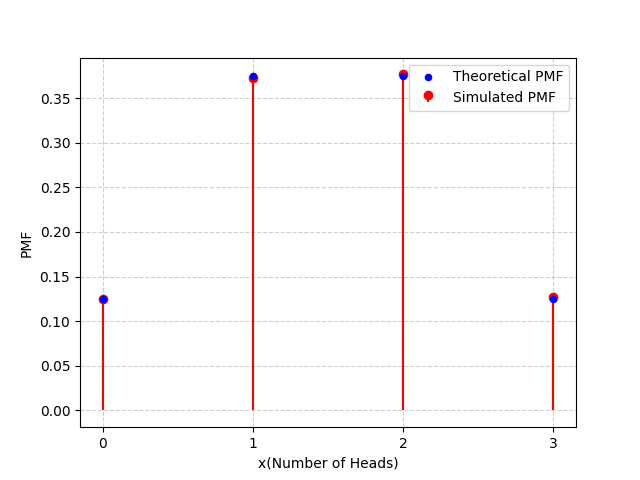
\includegraphics[width=\columnwidth]{figs/curve.png}
\end{figure}
\end{document}
